\chapter{Decision tree method}
Decision tree is a decision support tool that uses a tree-like model of decisions and their possible consequences, including chance event outcomes, resource costs, and utility. It is one way to display an algorithm that only contains conditional control statements.Decision trees are commonly used in operations research, specifically in decision analysis, to help identify a strategy most likely to reach a goal, but are also a popular tool in machine learning.

The decision tree is a flowchart-like structure in which each internal node represents a "test" on an attribute, each branch represents the outcome of the test, and each leaf node represents a class label (decision taken after computing all attributes). The paths from root to leaf (decision paths) represent classification rules.

A decision tree can be used to visually and explicitly represent decisions and decision making. The decisions are based on some conditions. There are several variants of DTs such as classification and regression trees (CART), chi-squared automatic interaction detection (CHAID) etc. The DT model used for this work is based on CART. 

\section{Classification and regression trees}
CART is a DT algorithm that produces binary classification or regression trees, depending on whether target variable is categorical or numeric. It can also be used to extract patterns or rules found in the dataset. Each tree node attempts to split the data in the most optimal manner so that the classification splits maximize the information gain. Figure \ref{fig:cart_illustration} illustrates a basic CART model.

\begin{figure}
    \centering
    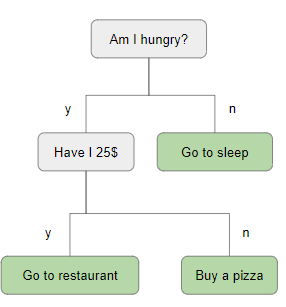
\includegraphics[scale=0.5]{chapters/images/cart_basic_example.png}
    \caption{A simple illustrative example for CART method \cite{edureka_decision_2018}.}
    \label{fig:cart_illustration}
\end{figure}

Each node in Figure \ref{fig:cart_illustration} represents a decision point. The decision at each node can be either True (yes) or False (No). Based on the decision we traverse to other decision points and ultimately reach the leaf node which is the final result. In this example, "Go to restaurant" is a final result which is recognised if "I am hungry" and "I have \$25".

The CART method has several advantages. First of all, it is simple to understand, interpret and visualize. It can handle both numerical and categorical data. CART decision trees require relatively a little effort from users for data preparation. These features make CART suitable for this work.

\section{Prediction and analysis}
The DT model has been applied for predicting the future values of passenger attributes based on previous observed values. This model is preferable because its structured rules are simple to follow and understand. Branches of DT shows the decisions that led to a given prediction. DT diagram also shows some interesting relationships between attributes. The results of the DT method are investigated after being applied to multiple target variables. Sample decision paths are shown in Figure \ref{fig:sample_dts}. The first one (left) shows the decision path where target variable is type of accident. It can be observed that, the age and the day of the accident are clearly significant factors in determining the nature of the accident. This is the main advantage of DT method. We will know how a particular decision is made. This can be visualized and might be useful in decision making process. 

\begin{figure}
   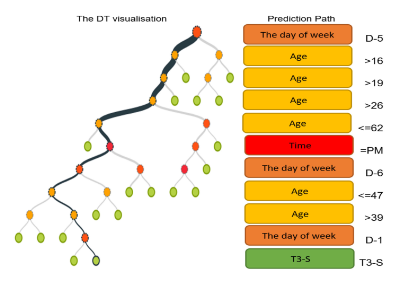
\includegraphics[width=0.475\textwidth]{chapters/images/dt_1.png}
   \hfill
   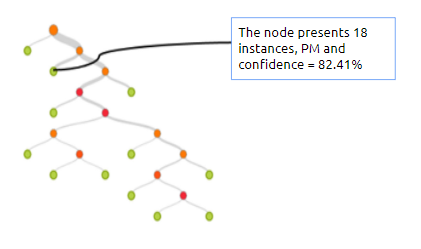
\includegraphics[width=0.475\textwidth]{chapters/images/dt_2.png}
   \caption{DT diagrams showing the prediction and data distribution from the training dataset.}
   \label{fig:sample_dts}
\end{figure}

Another important way to find trends from the data is the application of statistical tools on data. To determine the relationship between several variables, statistical plots like the scatter plot, histogram, etc. can be employed. For example the scatter plot in Figure \ref{fig:scatter_1} shows a relation between the details of the accidents and time with the passenger age. From the figure it is clear that PM has witnessed more accidents than AM. The relation between the details of the accidents and day of the week with the passenger age is depicted in Figure \ref{fig:scatter_2}. It can be observed that more accidents happen towards weekend. Histograms can be used to view the distribution of the data. As shown in the Figure \ref{fig:hist}, T1-F which corresponds to "falling from the train and struck by train" contributes to most of the fatalities happened in railway stations.

\begin{figure}
    \begin{minipage}[c]{0.4\linewidth}
        \centering
        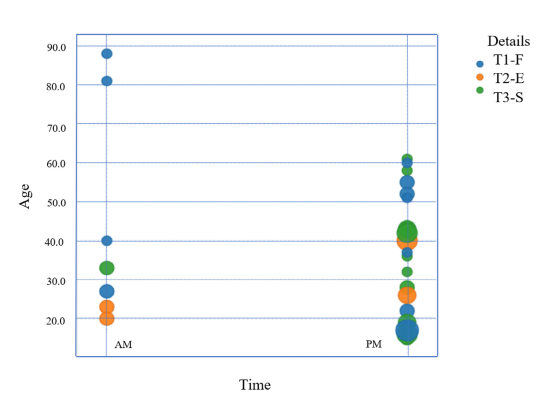
\includegraphics[scale=0.25]{chapters/images/scatter_1.png}
        \caption{Scatter plot showing a relation between the details of the accidents and time with the passenger age.}
        \label{fig:scatter_1}
    \end{minipage}
    \hfill
    \begin{minipage}[c]{0.40\linewidth}
        \centering
        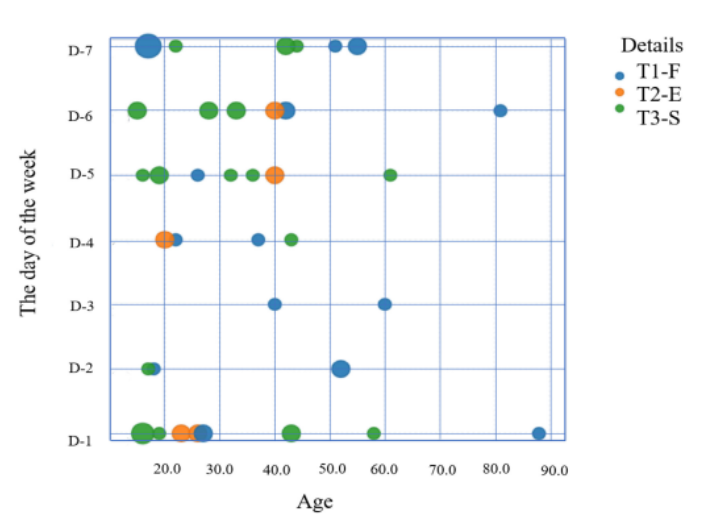
\includegraphics[scale=0.25]{chapters/images/scatter_2.png}
        \caption{Scatter plot showing the relation between the details of the accidents and day of the week with the passenger age.}
        \label{fig:scatter_2}
    \end{minipage}
\end{figure}


\begin{figure}
    \centering
    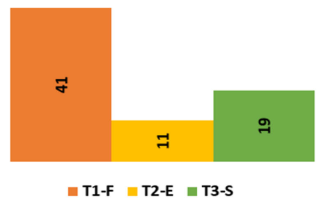
\includegraphics[scale=0.4]{chapters/images/hist.png}
    \caption{Histogram showing distribution of data}
    \label{fig:hist}
\end{figure}





